% Journal:
%   Journal of Ambient Intelligence and Smart Environments (JAISE), IOS Press
%   Web Intelligence and Agent Systems: An International Journal (wias)
%   Semantic Web: Interoperability, Usability, Applicability (SW)
% Latex 2e
% Test file iosart2c.tex

%[seceqn,secfloat,secthm,crcready]

% options: wias, jaise, sw
\documentclass{iosart2c}


\usepackage[T1]{fontenc}
\usepackage{times}%

\usepackage{natbib}
%\usepackage[dvips]{hyperref}
\usepackage{amsmath}
\usepackage{dcolumn}
%\usepackage{endnotes}
\usepackage{graphics}

%----- Another libraries ----
\usepackage[utf8]{inputenc}
\usepackage{todonotes}
\usepackage{hyperref}
\usepackage{paralist}
%----- Another libraries ----

\newcolumntype{d}[1]{D{.}{.}{#1}}


\firstpage{1} \lastpage{15} \volume{1} \pubyear{2015}


\begin{document}
\begin{frontmatter}                           % The preamble begins here.

%
%\pretitle{Pretitle}
\title{Dynamic LOD Cloud Diagram}

\review{Name Surname, University, Country}{Name Surname, University, Country}{Name Surname, University, Country}

\author{\fnms{Ciro} \snm{Baron Neto}}
,
\author{\fnms{Sebastian} \snm{Hellmann}}
,
\author{\fnms{Diego} \snm{Esteves}}
,
\author{\fnms{Luca} \snm{Matteis}}
,
\author{\fnms{Natanael} \snm{Arndt}}
,
\author{\fnms{Andre} \snm{Valdestilhas}}
\address{AKSW/BIS Universitat Leipzig,\\ Germany\\
E-mail: \{cbaron, hellmann, esteves, arndt, valdestilhas\}@informatik.uni-leipzig.de}

\begin{abstract}
The concept of Linked Open Data has been growing significantly, this growth comes with some problems such as data update and a way to filter them. This paper conducts a survey about approaches regarding the concept of LOD Cloud Diagram, a list of requirements and proposes an alternative solution that aims to provide a LOD Cloud Diagram updated in real time and allowing to apply make-filter on specific topics generating specific diagrams.
\end{abstract}

\begin{keyword}
Linked Open Data\sep Cloud Diagram\sep Semantic Web\sep
\end{keyword}

\end{frontmatter}


\section{Introduction}
Actually the current LOD Cloud image is generated and maintained by Richard Cyganiak from Centre for Data Analytics at NUI Galway and Anja Jentzsch form HPI company \cite{lodcloud2014}.
This Diagram is generated by one person, through sending emails and putting this information in a database.

The LOD Cloud Diagram \cite{lodcloud} is not updated and dosn't allow use of filters.

There is already previous research on the concept of LOD Cloud Diagram and Visualization of Linked Open Data, such as in \cite{Dadzie2011, IJST38378}, but this work is also intended to serve as a complement to this research.

\subsection{Directed link definition}
In order to provide a better explanation about the definition of the therm \"Directed Link\" that we use in this work, now will be explained in more details.

Let D = \{d1,d2,...,dn\} be a set of datasets in a RDF file.

We call a dataset linked if for two disjoint datasets di and dj the <some word...ask ciro or sebastian>:

d = \{<s,p,o>1, <s,p,o>2, ..., <s,p,o>n\} A dataset is a set of triples, where d is a Dataset and s is an subject, p is an  predicate and o is an object.

d_{oi} = \{o1, o2, o3, ..., on\} 

~Where~d_{oi}~is~ the~ list~ of~ objects.

d_{si} = \{s1, s2, s3, ..., sn\}

~Where~d_{si}~is~ the~ list~ of~ subjects.

count(d_{oi}~\bigcap~d_{sj}) >= 50

Then there is a directed link from d_{i}~to~d_{j}.

\subsection{Requirements}

\begin{itemize}
\item gathering information from various sources and try to us as much information as available in void, sd and co
\item generate dataid for each dataset
\item building a catalog of dataset meta-data
\item filtering by different properties of the datasets -> we should also ask claus and integrate facete (demo: \url{http://js.geoknow.eu/demos/jassa/pokedex-browser/}, \url{http://js.geoknow.eu/demos/jassa/sponate/sponate-castles.html} or even more complex: \url{http://js.geoknow.eu/demos/jassa-ui-angular/combination/app/})
\item Dynamic generation of cloud diagram picture
\item the picture could visualize more properties than just size, links and topic area (government, linguistic, social, geo, …) e.g. it could colorize the datasets by used language, set the size in proportion to how strongly it is interlinked, create a “heatmap” which visualizes, when the dataset was last updated, or any other property of the dataset
\end{itemize}

\section{Related Work and Existing approaches} %1,0 pages
\label{sec:related}

There are several existing approaches about Visualizing Data 2D, 3D, Flash, Flex, Mobile, among others \cite{SeveralSurveys}, \cite{Dadzie2011}, \cite{IJST38378}. This works are relevant to our work, but our main goal are more focused to LOD CLoud Diagram, in order to do a new Visualization of this Diagram that are updated and allow make-filters.

\subsection{lod-cloud.net: The Linking Open Data cloud diagram}
This work is our main motivation, because here we try to provide some improvements about the actual LOD Cloud Diagram \cite{lodcloud}.
The problems that we will try to provide some solution are: Up-to-dateness, because according the authors \cite{lodcloud}, \textbf{"This image shows datasets that have been published in Linked Data format, by contributors to the Linking Open Data community project and other individuals and organisations. It is based on metadata collected and curated by contributors to the Data Hub as well as on metadata extracted from a crawl of the Linked Data web conducted in April 2014."}.

Therefore, we can notice that this Graph is not updated automatically, because the last updated was: 2014-08-30, and of course, not allowing filters, because is an static image.


\subsection{VoID-graph}
VoID-graph \cite{Voidgraph} is a standalone web-tool that, given a VoID description, can visualize a diagram similar to the LOD cloud \cite{lodcloud}, is built using Open Web standards such as JavaScript, HTML5, CSS3 and SVG. Users can simply download the source-code and run the index.html file to utilize the tool from the webSite. Compared to other software, which requires the configuration of specific runtimes and the installation of a variety of dependencies, VoID-graph can more easily be hosted and installed on a variety of systems.

\subsection{LOD Cloud VoID Generator}
This work \cite{VoIdGenerator} is responsable by generate a VoID description of all datasets in the lodcloud group on the Data Hub.

This project is about generating a VoID description of all the datasets in the LOD Cloud diagram. It currently generates an RDF dump containing these descriptions, available online here:\footnote{\url{http://lod-cloud.net/data/void.ttl}}

The LOD Cloud diagram is a pictorial of datasets published in linked data format on the Web.
Metadata for these datasets is recorded in the Data Hub, an open directory of datasets. The lodcloud group contains metadata for all the datasets in the LOD Cloud diagram.
VoID is an RDF vocabulary for expressing metadata about such datasets in RDF format.
At some point, this project was intended to produce not just an RDF dump, but also RDF and HTML descriptions of each entity described in the dump. That effort stalled, and is removed from the current codebase, but can still be found in the feature-html branch.

Source-code for lod-cloud.net \cite{lodcloud}, can be found here:\footnote{ \url{https://github.com/lod-cloud/lod-cloud}}, the website of the Linked Open Data Cloud diagram \cite{lodcloud}.

\subsection{DataHub2Void}
There are an work \cite{Datahub2Void} that generates a VoID description of all datasets in the lodcloud group on the Data Hub.

\subsection{LOD for all}
This work \cite{lod4all} provides an LOD Cloud Diagram, that have some particularities, such as, when you keep you mouse pointer under an bubble, a kind of sub graph is showed. Allow make filters as well. Therefore this feature brings an easy way comparing with others that makes this work be relevant.
This work is licensed under a Creative Commons Attribution 3.0 Unported License. creative commons license. Copyright © 2014 FUJITSU LABORATORIES LTD.

Includes additional datasets beyond those that are officially part of the “lodcloud” group. Also include datasets that have been tagged with the “lod” tag (according to metadata collected from Datahub) and that follow the license criteria explained above.

Is interactive. You can filter datasets based on several criteria, zoom and pan around the diagram and select a dataset with a click to inspect its links to other datasets, or with a double-click to see the dataset details page.

\subsection{Towards a Dynamic Linked Data Observatory (DynLOD)}
The Dynamic Linked Data Observatory \cite{dynlod} is a framework to monitor Linked Data over an extended period of time. The core goal of our work is to collect frequent, continuous snapshots of a subset of the Web of Data that is interesting for further study and experimentation, with an aim to capture raw data about the dynamics of Linked Data. The resulting corpora will be made openly and continuously available to the Linked Data research community.

Until now, they provide weekly crawls and updated.

The newest crawl dumps should be available for download \footnote{\url{http://swse.deri.org/dyldo/data/}} roughly one day after they got crawled.

This work \cite{dynlod} proposes an way to monitoring Linked Open Data around the Web.
One possible problem is that data format, because we cannot found an specific format such as turtle, VoId Description or another one.

\subsection{Protovis} 
Protovis \cite{Protovis} was already been analysed before in \cite{SurveyLODDiagram1}, but as complement we can tell that is a graphical approach to visualizing the LOD Cloud diagram using free and open-source under the BSD License. It uses JavaScript and SVG for web-native visualizations and no plug-in required.
The Protovis team is now developing a new visualization library called D3.js \cite{d3js}, with improved support for animation and interaction.
There is no way filter and the graph is manually updated.

\subsection{Czech LOD Cloud}
Czech LOD (CzLOD) cloud diagram \cite{app24} show a set of interlinked LOD datasets that they have published in your research group trying to show the benefits of the Linked Data Visualization Model (LDVM) for LOD visualization.
The data are not automatic updated and we cannot found a way to make filters.

\subsection{lodlive} 
LODLive \cite{lodlive1} is an environment that generates an Graph based in some filter in some predefined dataSets like dbPedia.org and freebase.org, you also can input an URI.
This work allow make filters, but the result graph/Graph is not properly similar to LOD Cloud Diagram \cite{lodcloud}.
An suggestion maybe could be put a kind of automatically search for all datasets, could be direct in DataHub.io.

\subsection{rkbexplorer} 
The rkbexplorer \cite{rbkexplorer} presents a tool that provides an graphical environment. An good point is that according the literature \footnote{\url{http://lists.w3.org/Archives/Public/public-lod/2009Jan/0061.html}} that shows is  possible to generate a LOD Cloud Diagram using this tool and also allowing filters.

\subsection{Callimachus}
This work initiallly \cite{callimachus} is an tool for visualizing Linked Data, but still here because this tool can reproduce the LOD Cloud Diagram as well, but in his webSite \footnote{ \url{http://semanticweb.com/tag/callimachus-project}} is explained that is not a intention of this tool. Therefore, this is not a good way to adote this tool, unless we have only this way.

\subsection{Gephi: Semantic Web Crawling Visualization}
This approach \cite{WebCrawlVis} provide some examples and visualizations of semantic web crawls using Gephi \footnote{\url{http://gephi.github.io/}} as graph visualiser and LDSpider as semantic crawler, that allow filters, but not provide automatic update.
This work can be used as LOD Cloud Digram as well, because as lod-cloud.net use LDSpider to crawling the data.

%======== END OF RELATED WORKS ++++++++++++++++

\section{Criteria}
In order to provide a explanation about the criteria adopted in this work which allow to evaluate tools and approaches.

\paragraph{Data Updated Automatically:} The work needs to provide data that are automatically updated, in order to provide always an updated and reliable LOD Cloud Diagram.

\paragraph{Allow filter:} In order to provide an way to make sub LOD CLoud diagrams about specific subjects, for example, an sub LOD Cloud about Librarians. 

\begin{table}[htbp]
\caption{Selected approaches and criteria }
\begin{tabular}{|l|c|c|c|}
\hline
 & \multicolumn{ 3}{c|}{\textbf{Criteria}} \\ \hline
\multicolumn{1}{|c|}{\textbf{Approach / Tool}} & \textbf{Updated} & \textbf{Allow Filter} & \textbf{Web} \\ \hline
lod-cloud.net  &  &  & x \\ \hline
LOD for all &  & x & x \\ \hline
DynLOD & x &  & x \\ \hline
Protovis &  &  & x \\ \hline
VoID &  &  & x \\ \hline
LODLive &  & x &  \\ \hline
rkbexplorer &  & x & x \\ \hline
Callimachus &  & x & x \\ \hline
Gephi\\ Crawling Visualization &  & x &  \\ \hline
\end{tabular}
\label{Criteria}
\end{table}

\section{Linked Data Browsers}

Linked Data Browsers can be an way to visualise LOD-cloud diagrams, thus, the work by Dadzie 2011 \cite{Dadzie2011} shows key requirements and approaches, such as two tables represented by figures ~\ref{fig:crit1} and ~\ref{fig:crit2} that can represent some criteria comparing 15 tools to visualising Linked Data.

\begin{figure*}[tbp] 
  \centering
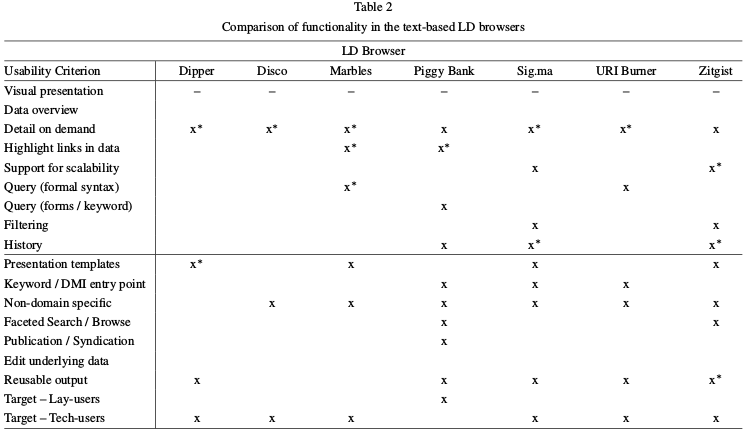
\includegraphics[width=\textwidth]{img/table2.png}
  \caption{Criteria about LD Browsers (1-2) \cite{Dadzie2011}}
  \label{fig:crit1}
\end{figure*}

\begin{figure*}[tbp] 
  \centering
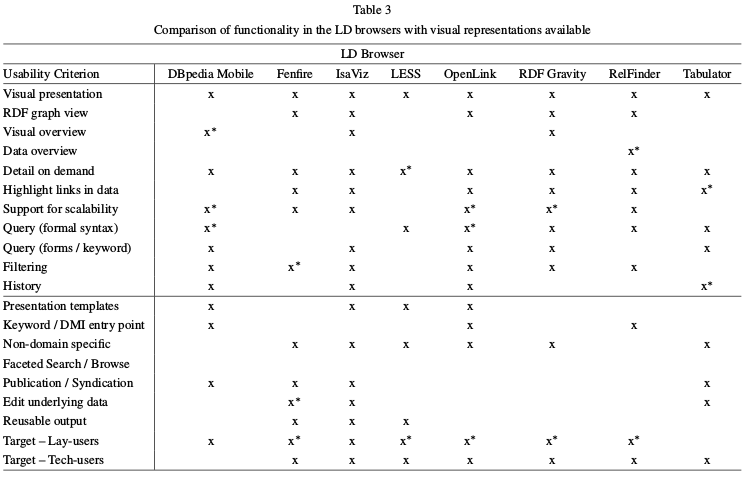
\includegraphics[width=\textwidth]{img/table3.png}
  \caption{Criteria about LD Browsers (2-2) \cite{Dadzie2011}}
  \label{fig:crit2}
\end{figure*}

\section{Steps to have you own LOD Cloud Diagram}

This steps are based in a tutorial provided by Luca Matteis \cite{Voidgraph} \footnote{\url{http://markmail.org/search/?q=+list\%3Aorg.w3.public-lod+lod+cloud+visualisation#query:lod\%20cloud\%20visualisation+page:1+mid:xiwz5envzoeqbq3x+state:results}}.

\begin{enumerate}

\item Download all metadata about datasets already stored in http://datahub.io/. Use this script:

\footnote{\url{https://github.com/lod-cloud/datahub2void}}

to get a void.ttl file

\item Load void.ttl into your RDF storage server.

\item Make this query:

PREFIX rdfs:<\url{http://www.w3.org/2000/01/rdf-schema#}> \\
PREFIX foaf:<http://xmlns.com/foaf/0.1/> \\
PREFIX tag:<\url{http://www.holygoat.co.uk/owl/redwood/0.1/tags/}> \\
PREFIX owl:<\url{http://www.w3.org/2002/07/owl#}> \\
PREFIX xsd:<\url{http://www.w3.org/2001/XMLSchema#}> \\
PREFIX void:<\url{http://rdfs.org/ns/void#}> \\
PREFIX rdf:<\url{http://www.w3.org/1999/02/22-rdf-syntax-ns#}> \\
PREFIX skos:<\url{http://www.w3.org/2004/02/skos/core#}> \\
PREFIX dcterms:<\url{http://purl.org/dc/terms/}>

select * { ?s a void:Linkset. ?s void:linkPredicate skos:exactMatch. ?s void:objectsTarget ?otarget. ?s void:subjectsTarget ?starget. ?s void:triples ?triples. }

\item Export results of this query as N-triples.
\item Download \url{https://github.com/lmatteis/void-graph}. 
\item Open file index.html in your browser. Inside text area field, paste all n-triples you have already exported. 

\item That is all. You must have your own LOD - Cloud in a couple seconds. 
\end{enumerate}

\section{Problem Analysis}

As stated in Section~\ref{sec:related} all of the tools we investigated have update intervals of over 4 months and need a lot of manual effort to keep meta data quality fresh.

We will use an short story in order to explain our contribution in a clear way.

\subsection{Story} 

I am a Greek Librarian and I want to find, filter and classify all datasets that is related to Greece (its people and locations), the greek language and any greek things (e.g. movies, books). Then I want to publish this classification and create my own LOD cloud images to help my colleagues (other Greek librarians) to browse all relevant datasets. I can spend the next three weeks full time to work on a software tool to plow through all the data.

\subsection{How to solve}
In order to solve this problem we provide an GUI that the user can find, filter and classify datasets this solution is called DataId-Graph, that cover an environment web where allows find, filter and classify your datasets in a easy and intuitive way create you own LOD cloud diagram, like the Figure~\ref{fig:greek} try to show.

\begin{figure*}[tbp] 
  \centering
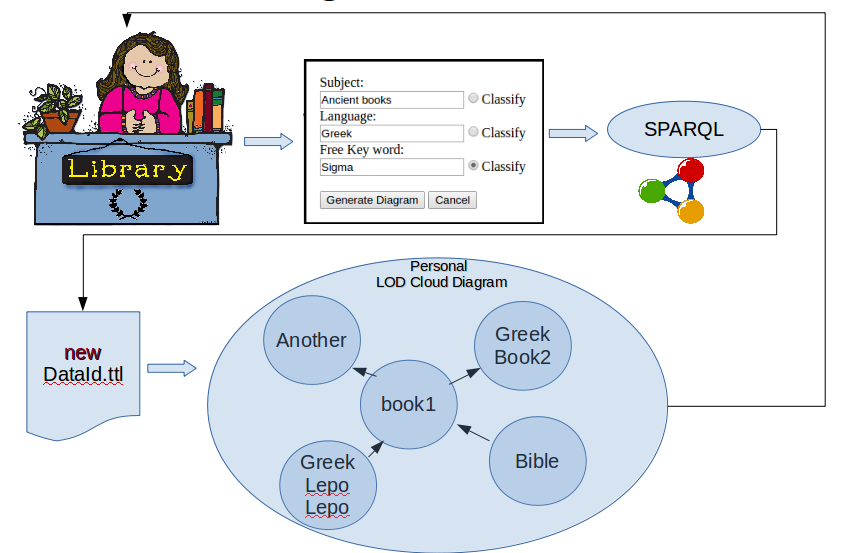
\includegraphics[width=\textwidth]{img/greeklib.png}
  \caption{Greek librarian case}
  \label{fig:greek}
\end{figure*}

\section{DataId}

DataID \cite{dataID2014} is an proposal of best-practice for LOD dataset descriptions which utilize RDF files hosted together with the datasets, under the same domain.
The data model is based on the widely used DCAT and VoID vocabularies, as well as supporting tools to create and publish DataIDs.
The DataID data model provides a uniform way to describe general metadata of datasets.

\begin{figure*}[tbp] 
  \centering
\includegraphics[width=\textwidth]{img/vocab.png}
  \caption{DataID vocabulary diagram}
  \label{fig:vocab}
\end{figure*}

The Figure~\ref{fig:vocab} shows the overall structure of DataID including the main features.


--> Semantics paper (ask Ciro);
Copy and paste from DataID paper ?

\subsection{How to index dataids for the new LOD Cloud image}


\subsection{Implementation}
We have five steps to complete the task as you can see in Figure~\ref{fig:idea2} that shows an fluxogram with all steps covered by our idea.

\begin{enumerate}
\item \textbf{Receive DataId:} In this step we will receive the DataId file, and do validations.
\item \textbf{Parse DataId:} After the reception of this DataId, it is possible to read and start to record the data, then we make a search for distributions.
\item \textbf{Check for modifications:} In this step we will use HTTP headers to find an signal that the data has modified, such as date or size.
\item \textbf{Compare Distributions:} Now we know that there are some modification, then, we need to compare distributions in order to know the right one, thus we use an probabilistic data structure called Bloom Filter \cite{bloomfilter} under DataId files to find modification on linksets and distributions.
\item \textbf{Update DataID:} In case of changes detected by BloomFilter, we provide an update under the DataId file, for exeample, Linksets, because the relations are based on linkesets, therefore, after update DataId file, but the main file remains with the same name, thus, the URL is the same, then we have an updated DataId-Graph.
\end{enumerate}

\begin{figure}
  \centering
  \includegraphics[width=\linewidth]{img/dlod5.png}
  \caption{Fluxogram about whole process.}
  \label{fig:idea2}
\end{figure}

\subsubsection{How Bloom Filters works}
The Bloom filter is an very important part of our work, because we can have an LOD Cloud Diagram updated and efficiently.

The Figure~\ref{fig:bloomfilter} shows an example of a Bloom filter, representing the set \{ x, y, z \}. The colored arrows show the positions in the bit array that each set element is mapped to. The element w is not in the set \{ x, y, z \}, because it hashes to one bit-array position containing 0. For this figure, m = 18 and k = 3.
\begin{figure}
  \centering
  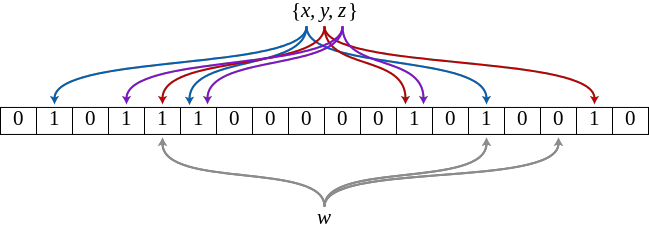
\includegraphics[width=\linewidth]{img/bloomfilter.png}
  \caption{Bloom filter.}
  \label{fig:bloomfilter}
\end{figure}

Explaining in more details, instead of set \{ x, y, z \} in our case we have set \{ Linkset1, Linkset2, ..., LinksetN \}. Then we will use this data structure to compare linksets and to know how many links we have among our DataId Files.

\subsection{DataID-Graph: Visualizing complex LOD DataSets}

The idea about Visualize Linked Datasets on the Web was originated by Lucas Matteis on his work called Void-graph. In this work we will provide some modifications that allows visualize DataID.
DataID complements the Void structure because DataID has VoId fields as well and privides an structure for representing Datasets more complete. <Ask MARTIN, CIRO, SEBASTIAN, DIEGO, etc..>

The Idea behind DataID \cite{dataID2014} is that can provides an structure to represent DataSets.
DataID is a best-practice for LOD dataset descriptions which utilize RDF files hosted together with the datasets, under the same domain. 
DataID has an data model, which is based on the widely used DCAT and VoID vocabularies, as well as supporting tools to create and publish DataIDs and use cases that show the benefits of providing semantically rich metadata for complex datasets.
One characteristic that makes possible to visualize DataID's as an Graph is the use of VoID vocabularies, this is the main feature that makes possible to visualise DataIDs, with some modifications in the VoID-graph \cite{Voidgraph} that will be explained in this paper.


\subsubsection{Architecture}
The architecture of DataID-graph is very similar to VoID-graph  \cite{Voidgraph}, as presented in Figure~\ref{fig:dataidgraph}.

\begin{figure}[t]
 \centering
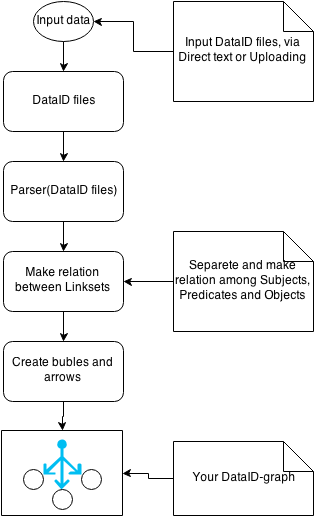
\includegraphics[height=9cm]{img/DataID-Graph.png}
  \caption{Activity Diagram for DataID-graph.}
  \label{fig:dataidgraph}
\end{figure}
------------------------>>>>>>

\section{LOD Cloud results}
--> Discuss with Ciro and Diego.

\section{Evaluation}
--> Discuss with Ciro and Diego.
(Discussion : Discuss ) (Andre)

Experimental evaluation: (Andre)

We can realize that our model present an improvement...

e.g. looking at the fact, that we could vizualize any property of the datasets: e.g. it could colorize the datasets by used language, set the size in proportion to how strongly it is interlinked, create a “heatmap” which visualizes, when the dataset was last updated, … this was not available so far and comes with a lot of work if done manually. With our (semi-)automatic approach nearly anything can be visualized

\begin{table}[htbp]
\caption{Evaluation}
\begin{tabular}{|l|l|l|l|l|}
\hline
\textbf{NameDataID} & \textbf{QtdTriples} & \textbf{TimeToCreate} & \textbf{\%FalsePositive} & \textbf{QtdLinksets} \\ \hline
x & x & x & x & x \\ \hline
\end{tabular}
\label{Evaluation}
\end{table}

\section{Some reasons for this work were identified as:}
\begin{enumerate}
\item Do something for people that no have enough knowledge about RDF nor Ontologies.
\item Visualising Data can help to identify errors.
\item Make Visual Queries and Filters without know SPARQL, because using SPARQL, before you need to understand the syntax and data content structure.
\end{enumerate}

\section{Summary of Contributions}
Here will provide an Summary explaining in a short and clean way the contributions that this work provided:
\begin{itemize}
\item \textbf{Dynamic LOD Cloud Diagram:} This work brings an LOD Cloud Diagram really updated and allowing filters, as we notice that does not exists an work that do the same thing.
\item \textbf{A survey:} In the Related works section you can see an updated survey about approaches regarding the concept of LOD Cloud Diagram, that compares and makes an short evaluation about this works. and we also provide a list of requirements.
\item \textbf{DataId-Graph} A way to visualize Datasets using VoId descriptions to represent an extension to the void-graph, because DataId-Graph shows an structure to describe datasets more complete than only VoId descriptions. DataId uses Void vocabularies as part of your structure, this feature makes possible to visualize DataId's. The source code \footnote{\url{https://github.com/firmao/void-graph.git}} about DataId-graph is available to download.
\item \textbf{Efficient comparison of linksets:} This part of work compare distributions in order to know the right one, thus we use an probabilistic data structure called Bloom Filter \cite{bloomfilter} with DataId files to find modification on linksets and distributions. Therefore we can notice, according Evaluation section that using Bloom filters we can have a better performance that justifies his use. This is an main point about this work, because without this performance that bloom filters brings to this work probably will be impracticable.

\end{itemize}


\section{Conclusions and Future Work} %0,5-1,0 pages
\label{sec:future}
Some conclusion...
-->> Future work: Use Radix tree to reduce de hard disk utilization.

\bibliographystyle{abbrv}
\bibliography{refs}


\end{document}